\documentclass[t]{beamer}
\usepackage{beamerthemesplit}
\usepackage{pstricks}
\usepackage{graphicx}
\usepackage{hyperref}
\usepackage{subfigure}
\usepackage{multirow}
\usepackage{listings}
\usepackage{courier}
\usepackage{xspace}

%\lstset{escapechar=@,style=customc}


\mode<presentation>
{ \usetheme{Boadilla}
  \setbeamercovered{transparent}
  \setbeamertemplate{items}[circle]
  \setbeamertemplate{theorems}[numbered]
  \setbeamertemplate{footline}[frame number]
}
 
%\useinnertheme[shadow=true]{rounded}
\useoutertheme{shadow}
\usecolortheme{whale}

\newcommand\blfootnote[1]{
  \begingroup
  \renewcommand\thefootnote{}\footnote{#1}
  \addtocounter{footnote}{-1}
  \endgroup
}

\mode
<all>

\title{C Programming: Lab 9}
\author{Wan-Lei Zhao}

\makeatletter
\DeclareRobustCommand\onedot{\futurelet\@let@token\@onedot}
\def\@onedot{\ifx\@let@token.\else.\null\fi\xspace}
\DeclareMathOperator*{\argmax}{argmax}
\makeatother

\begin{document}

\begin{frame}
   \begin{center}
    \vspace{24pt}
    \Huge\textbf{C Programming}\blfootnote{Contact: wlzhao@xmu.edu.cn}\\
     \Huge{\mbox{Lab 9: Pointers}}
    \vspace{36pt}
  \end{center}
  \begin{align*}
   \vspace{18pt}
      \large{\mbox{Lecturer:}~Dr.~\mbox{Wan-Lei~~Zhao}} \\
      \large{Spring~~Semester~~2022} \\
   \vspace{30pt}
  \end{align*}
\end{frame}

\definecolor{cornblue}{HTML}{6495ED}
\definecolor{navyblue}{HTML}{000080}
\definecolor{midnblue}{HTML}{191970}
\definecolor{lghtblue}{HTML}{B0C4DE}
\setbeamercolor{background}{fg=black, bg=lghtblue}
\setbeamercolor{palette primary}{fg=white, bg=lghtblue}
\setbeamercolor{palette secondary}{fg=black, bg=cornblue}
\setbeamercolor{palette tertiary}{fg=black, bg=lghtblue}
\setbeamercolor{palette quaternary}{fg=black, bg=lghtblue}
\setbeamercolor{frametitle}{fg=black, bg=white}
\definecolor{ballblue}{rgb}{0.13, 0.67, 0.8}
\definecolor{cornflowerblue}{rgb}{0.39,0.58,0.93}
\definecolor{babyblueeyes}{rgb}{0.63, 0.79, 0.95}

\setbeamertemplate{footline}
{
  \leavevmode%
  \hbox{%
  \begin{beamercolorbox}[wd=.275\paperwidth,ht=2.25ex,dp=1ex,center]{author in head/foot}%
    \usebeamerfont{author in head/foot}\insertshortauthor
  \end{beamercolorbox}%
  \begin{beamercolorbox}[wd=.44\paperwidth,ht=2.25ex,dp=1ex,center]{title in head/foot}%
    \usebeamerfont{title in head/foot}\insertshorttitle\hspace*{3em}
    \hspace*{1ex}
  \end{beamercolorbox}%
  \begin{beamercolorbox}[wd=.285\paperwidth,ht=2.25ex,dp=1ex,center]{date/foot}%
    \usebeamerfont{title in head/foot}\hspace*{2em}
    \insertframenumber{} / \inserttotalframenumber\hspace*{1ex}
  \end{beamercolorbox}}%
  \vskip0pt
}



% preset-listing options
\lstset{
  backgroundcolor=\color{white},   
  basicstyle=\footnotesize,    
  language=c,
  breakatwhitespace=false,         
  breaklines=true,                 % sets automatic line breaking
  captionpos=b,                    % sets the caption-position to bottom
  commentstyle=\color{ballblue},    % comment style
  extendedchars=true,              
  frame=single,                    % adds a frame around the code     
  keywordstyle=\color{blue},       % keyword style
  numbers=left,                    
  numbersep=5pt,                   
  numberstyle=\tiny\color{blue}, 
  rulecolor=\color{babyblueeyes},
  stepnumber=1,              
  stringstyle=\color{black},     % string literal style
  tabsize=4,                       % sets default tabsize to 4 spaces
  title=\lstname                   
}


\section{Pointer}
\label{sec:point}
\begin{frame}<beamer>
    \frametitle{Outline}
    \tableofcontents[currentsection]
\end{frame}

\begin{frame}
\frametitle{Pointer: flip (1)}
\begin{itemize}
	\item {Define a function to flip the elements of an array}
	\item {For instance:}
	a[7] =\{11, 4, 31, 2, 5, 12, 15\}
	\item {Change to}
	a[7] =\{15, 12, 5, 2, 31, 4, 11\}
\end{itemize}

\begin{itemize}
	\item {Requirements}
	\begin{enumerate}
	
		\item {Function looks like: \textcolor{blue}{void} \textbf{flip}(\textcolor{blue}{int} *a, \textcolor{blue}{int} sz)}
		\item {\textbf{*a} is the pointer pointing to array, \textbf{sz} is the length of array}
		\item {You should use pointer to visit the elements in the array}
		\item {Define a function \textcolor{blue}{void} \textbf{print}(\textcolor{blue}{int} *a, \textcolor{blue}{int} sz)}
		\item {Display the input array \textcolor{red}{before} and \textcolor{red}{after} you call \textbf{flip}}
	\end{enumerate}
\end{itemize}
\end{frame}


\begin{frame}
\frametitle{Pointer: flip (2)}
\vspace{-0.2in}
\begin{figure}
	\begin{center}
		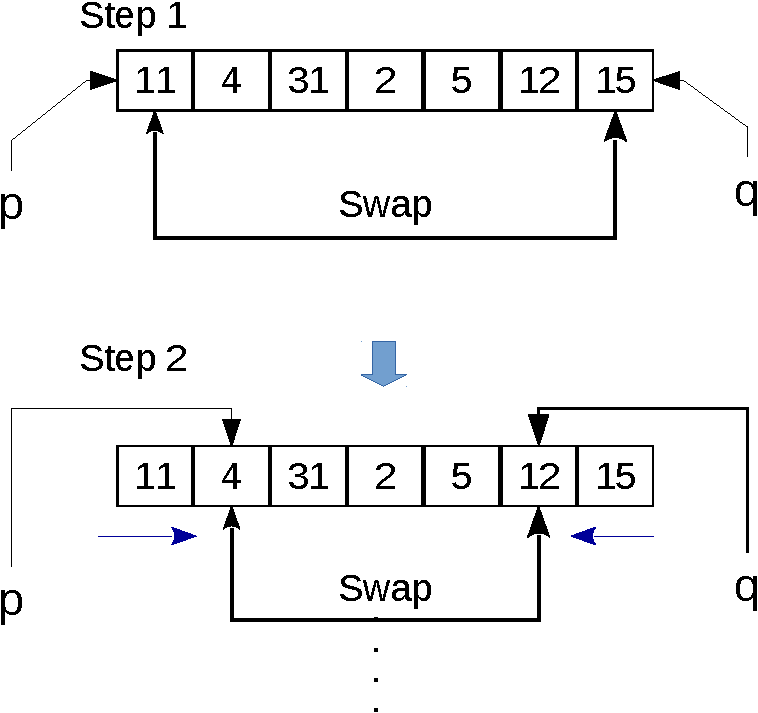
\includegraphics[width=0.65\linewidth]{figs/flip_demo.pdf}
	\end{center}
\end{figure}
\end{frame}

\ifx\answers\undefined
\begin{frame}[fragile]
\frametitle{Pointer: flip (3)}
\vspace{-0.2in}
\begin{columns}
\begin{column}{0.460\linewidth}
\begin{lstlisting}[xleftmargin=0.03\linewidth]
#include <stdio.h>
void flip(int *a, int sz)}
{
  int *ps = a, i = 0, t;
  int *pe = a+sz-1;
  for(i = 0; i < sz/2; i++)
  {
    t   = *ps;
    *ps = *pe;
    *pe = t;
  }
}
\end{lstlisting}
\end{column}
\begin{column}{0.52\linewidth}
\begin{lstlisting}[xleftmargin=0.03\linewidth, firstnumber=13]
void print(int *a, int sz)
{
   int *p = a, i;
   for(i = 0; i < sz; i++, p++)
   {
     printf("%d ", *p);
     printf("\n");
   }
}
int main()
{
 int a[7] ={11,4,31,2,5,12,15};
 print(a, 7);
 flip(a,  7);
 print(a, 7);
 return 0;
}
\end{lstlisting}
\end{column}
\end{columns}
\end{frame}
\fi

\begin{frame}
\frametitle{Count frequency of each character in a string (1)}

\begin{itemize}
	\item {Given a string char str[] ="abcesZzmwrlmAnersfdasaf"}
	\item {Count the number of ocurrence of each alphabet}
	\item {Upper case and lower case are viewed as the same}
	\item {Output non-zero ocurrences}
	\item {Hints}
	\begin{itemize}
		\item {Use an integer array of 26 length to keep the counts}
		\item {Try to implement toLower(char str[]) by yourself}
	\end{itemize}
\end{itemize}
\end{frame}

\ifx\answers\undefined
\begin{frame}[fragile]
\frametitle{Count frequency of each character in a string (2)}
\vspace{-0.25in}
\begin{columns}
\begin{column}{0.46\linewidth}
\begin{lstlisting}[xleftmargin=0.05\linewidth]
#include <stdio.h>
#include <ctype.h>
int main()
{
  char str[]="abcEsZzmwr";
  int *p = str, i = 0;
  int counts[26] = {0};
  toLower(str);
  while(*p != '\0')
  {
    i = *p-'a';
    counts[i]=counts[i]+1;
    p++;
  }

\end{lstlisting}
\end{column}
\begin{column}{0.54\linewidth}
\begin{lstlisting}[xleftmargin=0.05\linewidth]
  for(i = 0; i < 26; i++)
  {
    if(counts[i])
    printf("%c: %d\n", 'a'+i, counts[i]);
  }
  return 0;
}
\end{lstlisting}
\end{column}
\end{columns}
\end{frame}
\fi

\ifx\answers\undefined
\begin{frame}[fragile]
\frametitle{Count frequency of each character in a string (3)}
\begin{lstlisting}[xleftmargin=0.1\linewidth, linewidth=0.8\linewidth]
#include <stdio.h>
#include <ctype.h>
void toLower(char str[])
{
   char *p = str;
   while(*p != '\0')
   {
	  *p = tolower(*p);
	   p++;
   }
}
\end{lstlisting}
\begin{itemize}
	\item {Put this function before ``main()''}
	\item {\textbf{tolower}(\textcolor{blue}{char} ch): convert one character to lower case}
\end{itemize}
\end{frame}
\fi

\begin{frame}
\frametitle{Count frequency of each alphabet in a string (4)}

\begin{itemize}
	\item {How about the code is now case-sensitive}
	\item {Count the number of ocurrence of each alphabet}
	\item {Output non-zero ocurrences}
	\item {Hints}
	\begin{itemize}
		\item {Use an 2D integer array of 26{$\times$}2 length to keep the counts}
		\item {int counts[26][2]}
	\end{itemize}
\end{itemize}
\end{frame}


\section{File}
\label{sec:file}
\begin{frame}<beamer>
    \frametitle{Outline}
    \tableofcontents[currentsection]
\end{frame}

\begin{frame}
\frametitle{File operation}
\begin{itemize}
	\item {Open a file "hi.txt"}
	\item {Write down "hello this is \textbf{your name}"}
	\item {Close the file}
	\item {Hints}
	\begin{itemize}
		\item {FILE *fp = fopen("C:/MyDocuments/hi.txt", "w");}
		\item {fprintf(fp, "hello this is xxx");}
		\item {fclose(fp);}
	\end{itemize}
\end{itemize}
\end{frame}

\ifx\answers\undefined
\begin{frame}[fragile]
\frametitle{File operation: open and write}
\begin{lstlisting}[xleftmargin=0.08\linewidth, linewidth=0.9\linewidth]
#include <stdio.h>
int main()
{
  char str[]="hello this is xxx";
  FILE *fp = fopen("C:/MyDocuments/hi.txt", "w");
  if(fp == NULL)
  {
    printf("File cannot open!\n");
    return 0;
  }
  fprintf(fp, str);
  fclose(fp);
}
\end{lstlisting}

\end{frame}
\fi

\ifx\answers\undefined
\begin{frame}[fragile]
\frametitle{File operation: open and read}
\begin{lstlisting}[xleftmargin=0.08\linewidth,linewidth=0.9\linewidth]
#include <stdio.h>
int main()
{
  char str[64]="";
  FILE *fp = fopen("C:/MyDocuments/hi.txt", "r");
  if(fp == NULL){
   printf("File cannot open!\n");
   return 0;
  }
  fscanf(fp, str);}
  fclose(fp);
  printf("%s\n", str);
}
\end{lstlisting}
\end{frame}
\fi


\end{document}
